\documentclass[12pt,letterpaper]{article}
\usepackage[spanish,es-tabla]{babel}
\usepackage{fontspec}
\setmainfont{Latin Modern Roman}
\usepackage[margin=2.5cm]{geometry}
\usepackage{graphicx,booktabs,amsmath,array,hyperref,fancyhdr,longtable}

\hypersetup{colorlinks=true,linkcolor=black,urlcolor=blue}
\linespread{1.12}\setlength{\parindent}{0pt}
\setlength{\parskip}{6pt}
\setlength{\emergencystretch}{3em}
\pagestyle{fancy}\fancyhf{}\fancyhead[L]{\small Comparación de bases de datos} \fancyhead[R]{\small Producción agrícola}\fancyfoot[C]{\thepage}\renewcommand{\headrulewidth}{0.3pt}\setlength{\headheight}{14pt}
\begin{document}
\begin{titlepage}\centering
{\Large\bfseries Universidad Politécnica de Chiapas\par}\vspace{0.5cm}
{\large Ingeniería en Tecnologías de la Información e Innovación Digital\par}
\vfill
{\large Actividad: Bases de datos orientadas a documentos\par}\vspace{0.9cm}
{\LARGE\bfseries Rendimiento de bases de datos documentales: caso de producción agrícola\par}\vspace{0.5cm}
{\large Comparación entre MongoDB y PostgreSQL\par}
\vfill
\begin{tabular}{rl}
Materia: & Base de datos en la nube \\
Docente: & Horacio Irán Solís Cisneros \\
Alumno: & Uzzi Yazziel Gonzaga Gómez \\
Matrícula: & 243734 \\
Fecha: & 01 de noviembre de 2026
\end{tabular}
\vspace{2cm}\end{titlepage}
\pagenumbering{roman}\tableofcontents\clearpage\listoftables\listoffigures\clearpage\pagenumbering{arabic}

\section*{Resumen}
\addcontentsline{toc}{section}{Resumen}
Se compararon MongoDB y PostgreSQL JSONB con datos sintéticos de cosechas bajo tres límites de CPU y memoria. La matriz contiene 162 registros: 128 con estado \texttt{ok}, 21 con \texttt{spill}, 12 con \texttt{error} y uno con \texttt{oom}. Estos estados se conservaron tal como se registraron. Una corrida con error tiene el indicador de spill desconocido porque faltaron registros del profiler.

En Q1 con perfil A y un cliente, la mediana de las tres corridas fue 0,853 consultas por segundo para MongoDB y 0,570 para PostgreSQL. En Q2, para ese mismo perfil y concurrencia, PostgreSQL registró mayor rendimiento en las variantes medidas. Son resultados de este conjunto y configuración: no demuestran que exista un motor mejor para cualquier aplicación.


\section*{Introducción y objetivos}
\addcontentsline{toc}{section}{Introducción y objetivos}
La actividad compara dos maneras de consultar información organizada como documentos: una base documental y una base relacional que guarda documentos JSON. Para adaptar el ejemplo del manual, el escenario elegido es el registro de cosechas agrícolas. Una cosecha contiene datos de ubicación y una lista de lotes; cada lote representa un cultivo y una cantidad producida. Los datos fueron generados para el experimento, no proceden de productores reales.

El objetivo general es observar cómo responden MongoDB y PostgreSQL cuando se ejecutan consultas equivalentes con recursos limitados. La comparación incluye el número de consultas terminadas, el tiempo de respuesta, la presión sobre el procesador y la memoria, y los casos en que se utilizó disco temporal o se produjo una falla. El objetivo no es escoger un ganador para cualquier aplicación, sino explicar qué ocurrió bajo las condiciones de esta prueba.

Las tres preguntas del manual orientan el análisis. La primera (M1) trata sobre el cambio en los tiempos de respuesta cuando varían los recursos y el número de clientes. La segunda (M2) examina el manejo de memoria para ordenar o agrupar, junto con los casos de uso de disco y falta de memoria. La tercera (M3) solicita el consumo por cada 1.000 documentos procesados. En este último punto se presentan las mediciones disponibles y se explica por qué no fue posible obtener una cifra fiable por documento.

El caso agrícola mantiene la estructura de la actividad: medio millón de registros, listas anidadas, dos cargas de consulta, tres perfiles de recursos y varias concurrencias. Las cantidades y resultados del documento de ejemplo del profesor corresponden a otro dominio y no se trasladaron a esta evaluación.

\section*{1. Equipo y entorno}
\addcontentsline{toc}{section}{1. Equipo y entorno}
El experimento se ejecutó en un equipo con Intel Core i7-13620H, 15,64 GiB de memoria utilizable, Windows 11 y Ubuntu 24.04.3 sobre WSL2. Se utilizaron Docker Desktop 4.55.0 y Docker Engine 29.1.3. Los motores fueron MongoDB 9.0.4 y PostgreSQL 18.6; las imágenes y sus identificadores están fijados en \texttt{protocolo.json}.

Los motores se ejecutaron por separado, con datos en volúmenes de Docker. Los límites fueron: A, 4 CPU y 4096 MiB; B, 2 CPU y 2048 MiB; C, 1 CPU y 1024 MiB. El intercambio de memoria del contenedor se limitó a cero. Se usaron cAdvisor, Node Exporter y Prometheus para recopilar métricas. Las comprobaciones de infraestructura están en \texttt{resultados/\allowbreak{}verificacion\_\allowbreak{}fase1.json}.


\subsection*{Cómo interpretar los perfiles}
El perfil A dispone de cuatro unidades de CPU y 4.096 MiB de memoria; sirve como referencia dentro del experimento. El perfil B reduce ambos límites a la mitad y el C los reduce a una cuarta parte. La palabra referencia no garantiza ausencia completa de interferencias: Windows, WSL2, los servicios de monitoreo y el estado del equipo también pueden afectar las mediciones.

Los límites se aplicaron a los contenedores, no equivalen a reservar de forma exclusiva todo el equipo para un motor. La comparación entre perfiles debe considerar que CPU y memoria cambian al mismo tiempo. Por ello, una diferencia entre A y C por sí sola no permite atribuir el cambio únicamente al procesador o únicamente a la memoria.

La restricción del procesador (throttling) registra tiempo acumulado en que el contenedor alcanzó el límite de CPU impuesto. Valores altos indican presión relacionada con ese límite, pero no establecen por sí mismos la causa completa de una latencia. La memoria residente (RSS) es una medida de memoria asociada al contenedor; no representa necesariamente toda la memoria utilizada por el sistema ni permite comparaciones independientes de las herramientas empleadas.

\section*{2. Datos, consultas y método}
\addcontentsline{toc}{section}{2. Datos, consultas y método}
Se generaron 500.000 cosechas sintéticas con 1.499.983 lotes, derivados de forma determinista del conjunto inicial. Cada cosecha contiene productor, ubicación y una lista de lotes con cultivo, cajas y kilogramos por caja. El total es la suma de cajas por kilogramos por caja. El umbral de 50 kg por caja es una condición artificial del experimento, no una descripción de prácticas agrícolas reales.

Para identificar el archivo de datos se calculó una huella digital (SHA-256). Esta cadena permite comprobar si una copia conserva exactamente el mismo contenido que el archivo registrado; su valor completo se incluye en la sección de evidencia. Se verificaron 500.000 registros en cada motor y 199.729 cosechas que cumplen el filtro temporal y de estado. Esta comprobación no prueba por sí sola la igualdad exhaustiva de todos los documentos.

Q1 desanida los lotes, selecciona aquellos con más de 50 kg por caja y agrupa producción total y promedio por país y cultivo. Q2 filtra cosechas finalizadas desde el 1 de enero de 2026 y obtiene las 1.000 con mayor peso. Se evaluaron las opciones de disco de MongoDB y \texttt{work\_\allowbreak{}mem} de 4 MB y 64 MB en PostgreSQL para Q2. El conjunto expandido tiene 54 escenarios y tres repeticiones por escenario: 162 registros. La ampliación de variantes frente a las 36 celdas base del manual es una decisión del proyecto.

Cada repetición programó 60 segundos de calentamiento, 300 de medición y 60 de enfriamiento, con 1, 10 o 50 clientes. La cantidad de consultas completadas por segundo se expresa como rendimiento (QPS). Para describir los tiempos de respuesta se usan medidas que indican qué proporción de consultas terminó dentro de cierto tiempo (percentiles): el P95 deja al 95 \% de las consultas medidas en ese tiempo o menos, y el P99 deja al 99 \%. Los percentiles se calcularon con operaciones que comenzaron y terminaron dentro de la ventana; 2.991 operaciones cruzaron el cierre en el conjunto completo y no entran en esos percentiles. Esta regla puede dejar fuera consultas largas, por lo que no se deben comparar los P99 sin considerar esa limitación.

La validación funcional detallada encontró 20 grupos Q1 con sumas y conteos exactos. La mayor diferencia de promedio fue 5,23 × 10$^{-14}$ y quedó dentro de la tolerancia documentada. Las cuatro variantes Q2 produjeron los mismos 1.000 pesos en orden. El corte fue 2.719 kg y hay 998 cosechas por encima; un identificador difirió entre motores en el empate del corte. Evidencia: \texttt{resultados/\allowbreak{}validacion\_\allowbreak{}agricola\_\allowbreak{}detallada.json}. La validación de consultas no equivale a una comparación exhaustiva de todas las filas almacenadas.

El umbral de diferencia de ritmo del reloj fue menor a 2,5 \%. El límite de huecos interiores de telemetría cambió durante la matriz: 2,5 segundos para las primeras 16 corridas, 4 segundos para las siguientes 45 y 6 segundos desde el escenario 62; se mantuvo una cobertura mínima del 90 \%. Son decisiones del proyecto, no límites comprobados del profesor. Un intervalo sin muestras puede ocultar picos breves. Para diagnosticar spill se utilizó el profiler de MongoDB, cuya instrumentación añade carga. Su colección creció de 1 MiB a 256 MiB después de la corrida 82; esto puede afectar la comparación entre etapas.


\subsection*{Cómo se adaptó el caso de uso}
En el manual, cada orden contiene artículos con cantidades y precios. En el caso agrícola, el registro principal es una cosecha y la lista anidada contiene lotes. El productor y su ubicación cumplen el papel de los datos de cliente y ubicación; el cultivo permite agrupar de forma similar a la categoría. En lugar de importe económico se estudia el peso producido: cajas multiplicadas por kilogramos por caja.

Por ejemplo, si un lote hipotético contiene dos cajas de 60 kg, aporta 120 kg al grupo de su país y cultivo. Ese ejemplo solo explica la operación y no representa un dato observado. La condición de más de 50 kg por caja reproduce la forma del filtro del manual; es una regla sintética y no pretende describir una práctica agrícola habitual.

Q1 recorre la lista de lotes, aplica el filtro y agrupa los resultados. Para cada país y cultivo calcula el peso total, el promedio por lote y el número de lotes. Esta consulta permite observar el trabajo de recorrer y agrupar elementos anidados. Q2 selecciona cosechas finalizadas desde el inicio de 2026, las ordena por peso total y devuelve las 1.000 más pesadas. Ambas consultas se expresaron para MongoDB y PostgreSQL con el mismo objetivo lógico.

Para Q2 se probaron dos opciones en cada motor. En MongoDB se permitió o se impidió el uso de disco; en PostgreSQL se usaron 4 MB y 64 MB como límite de memoria de trabajo por operación. Estos controles no son equivalentes: habilitar disco no significa asignar 64 MB. Por eso el informe identifica cada variante y evita presentar las parejas como si fueran idénticas.

\subsection*{De una celda a sus resultados}
Una celda combina motor, perfil, consulta, variante cuando corresponde y número de clientes. Cada celda se repitió tres veces. Las variantes adicionales de Q2 amplían la matriz base del manual hasta 54 escenarios y 162 registros. Cada repetición programó un periodo de preparación, uno de medición y uno de cierre; los tres duraron 60, 300 y 60 segundos respectivamente.

La velocidad de trabajo (QPS) indica cuántas consultas se completaron por segundo. El tiempo que tarda una consulta en terminar se conoce como latencia. El P95 y el P99 describen, respectivamente, el tiempo dentro del cual terminó el 95 \% y el 99 \% de las consultas incluidas. Se calcula cada medida por repetición y después se toma el valor central (mediana). No se juntaron todas las consultas de las tres repeticiones para calcular un único percentil.

Cada resultado conserva su estado: \texttt{ok} indica que no se registró spill ni un fallo; \texttt{spill} indica uso de disco temporal detectado; \texttt{error} identifica una falla de la corrida o de su evidencia; y \texttt{oom} señala falta de memoria detectada. Un resultado con spill no debe confundirse con un fallo: puede completar consultas usando disco. Los errores y el caso OOM permanecen en los datos, aunque no se emplean para construir las medianas de rendimiento.

\subsection*{Comprobación de equivalencia}
Antes de interpretar la velocidad es necesario verificar que las consultas hagan un trabajo comparable. Se comprobaron los recuentos generales y los resultados de Q1 y Q2. En Q1 coincidieron exactamente los conteos y las sumas de los 20 grupos. La diferencia máxima de promedio fue muy pequeña y quedó dentro de la tolerancia numérica documentada, que contempla diferencias de representación de decimales.

En Q2 las cuatro variantes devolvieron los mismos 1.000 pesos ordenados. En el límite hubo cosechas empatadas en 2.719 kg y por ello los identificadores seleccionados por los motores no fueron todos iguales: coincidieron 999. El empate permite esa diferencia sin que cambie la lista de pesos. Estas comprobaciones respaldan la equivalencia de las consultas probadas, pero no constituyen una comparación exhaustiva de cada campo de los 500.000 registros.

\subsection*{Lectura de la evidencia de rendimiento}
El P99 puede variar considerablemente si hay pocas consultas completas. En 26 corridas utilizables hubo menos de 100 tiempos completos, por lo que una observación puede cambiar de forma notable el resultado. Además, 2.991 operaciones atravesaron el cierre de la ventana en toda la matriz y no entraron en los percentiles. Es importante no interpretar los valores como si incluyeran todas las consultas largas.

La captura de métricas también tiene límites. El intervalo máximo permitido sin muestras interiores cambió de 2,5 a 4 y después a 6 segundos; la cobertura mínima se mantuvo en 90 \%. El cambio debe tenerse en cuenta al comparar etapas. La herramienta de diagnóstico de MongoDB agregó carga y su colección pasó de 1 MiB a 256 MiB después de la corrida 82. Una corrida perdió registros de diagnóstico y su uso de disco quedó desconocido. Estos puntos se conservan para que el lector pueda valorar la evidencia.

\section*{3. Resultados consolidados}
\addcontentsline{toc}{section}{3. Resultados consolidados}
El valor central de las repeticiones ordenadas (mediana) resume cada escenario. Las medianas siguientes se calculan sobre las repeticiones con estado \texttt{ok} o \texttt{spill}; los estados \texttt{error} y \texttt{oom} se mantienen en el CSV original. El resumen completo, con número de repeticiones, mínimo y máximo por escenario, está en \texttt{resultados/\allowbreak{}resumen\_\allowbreak{}agricola.csv}. Cinco escenarios tienen menos de tres repeticiones utilizables. El QPS es consultas por segundo; las latencias están en milisegundos.

\par\begin{minipage}{\textwidth}\refstepcounter{table}\addcontentsline{lot}{table}{\protect\numberline{\thetable}Resultados seleccionados con perfil A}\begin{center}\textbf{Tabla \thetable. Resultados seleccionados con perfil A}\par\small\resizebox{\textwidth}{!}{\begin{tabular}{llrrr}\toprule
Perfil A, 1 cliente & Motor & Mediana QPS & Mediana P95 (ms) & Mediana P99 (ms) \\ \midrule
Q1 & MongoDB & 0,853 & 1.209,6 & 1.252,2 \\ 
Q1 & PostgreSQL & 0,570 & 1.814,4 & 1.852,9 \\ 
Q2 sin disco / 4 MB & MongoDB & 2,667 & 408,3 & 429,1 \\ 
Q2 sin disco / 4 MB & PostgreSQL & 9,870 & 111,0 & 127,0 \\ 
Q2 con disco / 64 MB & MongoDB & 2,647 & 413,5 & 431,1 \\ 
Q2 con disco / 64 MB & PostgreSQL & 9,663 & 114,4 & 124,6 \\ 
\bottomrule\end{tabular}}\end{center}\end{minipage}
Las opciones de Q2 son tratamientos distintos, no configuraciones equivalentes entre motores. La comparación debe leerse junto con los límites y los planes, y no atribuirse a una sola causa. En Q1 con perfil A y 50 clientes, las medianas de P99 fueron 36.105,7 ms en MongoDB y 166.957,9 ms en PostgreSQL; estas cifras no eliminan la advertencia sobre operaciones que cruzaron la ventana.

En PostgreSQL Q1 con 50 clientes y perfil B se registraron dos errores y un OOM; con perfil C hubo tres errores. En MongoDB Q2 con 50 clientes y perfil C, ambas variantes registraron tres errores cada una. No hay medianas de rendimiento utilizables para esos cuatro escenarios. El quinto escenario incompleto es MongoDB A, Q2 sin disco, 10 clientes: dos \texttt{ok} y un \texttt{error} por evidencia de profiler incompleta. No se interpretó su spill desconocido como falso.

En 26 corridas con estado \texttt{ok} o \texttt{spill} hubo menos de 100 latencias completas en la ventana. En ellas el P99 es especialmente sensible a una sola observación. Los contadores OOM deben interpretarse mediante su cambio durante la ventana, no solo por un valor acumulado. El caso OOM de PostgreSQL B/Q1/50 mostró un incremento de \texttt{oom\_\allowbreak{}kill} de 1 a 2 durante la corrida.

\subsection*{Resultados por escenario}
Las tablas siguientes amplían la comparación a los 54 escenarios. Cada fila muestra el valor central de las repeticiones utilizables (ok o spill), junto con la cantidad de repeticiones que lo integran. El guion indica que no hubo una mediana utilizable; no significa que la consulta tardó cero. El tiempo de restricción de CPU es acumulado y puede superar los 300 segundos de la ventana.
\par\begin{minipage}{\textwidth}\refstepcounter{table}\addcontentsline{lot}{table}{\protect\numberline{\thetable}Resumen de MongoDB con perfil A}\begin{center}\textbf{Tabla \thetable. Resumen de MongoDB con perfil A}\par\small\begin{tabular}{llrrrrr}\toprule Consulta & Clientes & N & QPS & P95 ms & P99 ms & CPU s \\ \midrule
Q1 & 1 & 3/3 & 0,85 & 1209,6 & 1252,2 & 0,0 \\
Q1 & 10 & 3/3 & 2,15 & 4995,5 & 5111,7 & 1814,9 \\
Q1 & 50 & 3/3 & 1,64 & 34302,3 & 36105,7 & 3522,2 \\
Q2\_DISK & 1 & 3/3 & 2,65 & 413,5 & 431,1 & 0,0 \\
Q2\_DISK & 10 & 3/3 & 8,17 & 1371,7 & 1435,4 & 1806,1 \\
Q2\_DISK & 50 & 3/3 & 6,71 & 11892,5 & 14191,6 & 3573,5 \\
Q2\_NO\_DISK & 1 & 3/3 & 2,67 & 408,3 & 429,1 & 0,0 \\
Q2\_NO\_DISK & 10 & 2/3 & 8,14 & 1382,2 & 1472,0 & 1808,0 \\
Q2\_NO\_DISK & 50 & 3/3 & 6,75 & 11706,8 & 13695,0 & 3565,3 \\
\bottomrule\end{tabular}\end{center}\end{minipage}\par
\par\begin{minipage}{\textwidth}\refstepcounter{table}\addcontentsline{lot}{table}{\protect\numberline{\thetable}Resumen de MongoDB con perfil B}\begin{center}\textbf{Tabla \thetable. Resumen de MongoDB con perfil B}\par\small\begin{tabular}{llrrrrr}\toprule Consulta & Clientes & N & QPS & P95 ms & P99 ms & CPU s \\ \midrule
Q1 & 1 & 3/3 & 0,87 & 1195,7 & 1221,5 & 0,4 \\
Q1 & 10 & 3/3 & 1,09 & 9899,1 & 10095,4 & 2429,2 \\
Q1 & 50 & 3/3 & 0,84 & 66195,5 & 69897,8 & 4103,7 \\
Q2\_DISK & 1 & 3/3 & 2,69 & 409,3 & 429,0 & 0,4 \\
Q2\_DISK & 10 & 3/3 & 4,01 & 2805,7 & 3000,1 & 2437,1 \\
Q2\_DISK & 50 & 3/3 & 3,40 & 24600,8 & 30197,7 & 4164,0 \\
Q2\_NO\_DISK & 1 & 3/3 & 2,69 & 404,8 & 418,8 & 0,4 \\
Q2\_NO\_DISK & 10 & 3/3 & 4,06 & 2795,6 & 2979,5 & 2445,0 \\
Q2\_NO\_DISK & 50 & 3/3 & 3,42 & 24095,9 & 29799,9 & 4167,4 \\
\bottomrule\end{tabular}\end{center}\end{minipage}\par
\par\begin{minipage}{\textwidth}\refstepcounter{table}\addcontentsline{lot}{table}{\protect\numberline{\thetable}Resumen de MongoDB con perfil C}\begin{center}\textbf{Tabla \thetable. Resumen de MongoDB con perfil C}\par\small\begin{tabular}{llrrrrr}\toprule Consulta & Clientes & N & QPS & P95 ms & P99 ms & CPU s \\ \midrule
Q1 & 1 & 3/3 & 0,80 & 1316,8 & 1631,0 & 13,5 \\
Q1 & 10 & 3/3 & 0,50 & 21688,0 & 22195,1 & 2783,1 \\
Q1 & 50 & 3/3 & 0,48 & 131996,8 & 142992,6 & 4326,3 \\
Q2\_DISK & 1 & 3/3 & 0,33 & 3396,4 & 3557,2 & 15,6 \\
Q2\_DISK & 10 & 3/3 & 0,49 & 29490,6 & 30498,0 & 2008,0 \\
Q2\_DISK & 50 & 0/3 & -- & -- & -- & -- \\
Q2\_NO\_DISK & 1 & 3/3 & 0,33 & 3411,4 & 3590,6 & 15,9 \\
Q2\_NO\_DISK & 10 & 3/3 & 0,34 & 36593,1 & 37803,1 & 2212,2 \\
Q2\_NO\_DISK & 50 & 0/3 & -- & -- & -- & -- \\
\bottomrule\end{tabular}\end{center}\end{minipage}\par
\par\begin{minipage}{\textwidth}\refstepcounter{table}\addcontentsline{lot}{table}{\protect\numberline{\thetable}Resumen de PostgreSQL con perfil A}\begin{center}\textbf{Tabla \thetable. Resumen de PostgreSQL con perfil A}\par\small\begin{tabular}{llrrrrr}\toprule Consulta & Clientes & N & QPS & P95 ms & P99 ms & CPU s \\ \midrule
Q1 & 1 & 3/3 & 0,57 & 1814,4 & 1852,9 & 0,0 \\
Q1 & 10 & 3/3 & 0,47 & 38923,2 & 42999,7 & 236,9 \\
Q1 & 50 & 3/3 & 0,18 & 166957,9 & 166957,9 & 181,4 \\
Q2\_4MB & 1 & 3/3 & 9,87 & 111,0 & 127,0 & 0,0 \\
Q2\_4MB & 10 & 3/3 & 7,21 & 2395,9 & 2500,6 & 2531,0 \\
Q2\_4MB & 50 & 3/3 & 6,90 & 9294,2 & 9805,7 & 2849,7 \\
Q2\_64MB & 1 & 3/3 & 9,66 & 114,4 & 124,6 & 0,0 \\
Q2\_64MB & 10 & 3/3 & 7,23 & 2394,0 & 2497,1 & 2482,0 \\
Q2\_64MB & 50 & 3/3 & 6,89 & 9213,3 & 9697,4 & 2847,6 \\
\bottomrule\end{tabular}\end{center}\end{minipage}\par
\par\begin{minipage}{\textwidth}\refstepcounter{table}\addcontentsline{lot}{table}{\protect\numberline{\thetable}Resumen de PostgreSQL con perfil B}\begin{center}\textbf{Tabla \thetable. Resumen de PostgreSQL con perfil B}\par\small\begin{tabular}{llrrrrr}\toprule Consulta & Clientes & N & QPS & P95 ms & P99 ms & CPU s \\ \midrule
Q1 & 1 & 3/3 & 0,27 & 5315,3 & 7109,1 & 30,3 \\
Q1 & 10 & 3/3 & 0,14 & 92876,3 & 94892,0 & 135,1 \\
Q1 & 50 & 0/3 & -- & -- & -- & -- \\
Q2\_4MB & 1 & 3/3 & 5,44 & 199,1 & 211,0 & 475,3 \\
Q2\_4MB & 10 & 3/3 & 3,46 & 4999,2 & 5202,5 & 2922,8 \\
Q2\_4MB & 50 & 3/3 & 3,37 & 19298,2 & 20600,1 & 3313,7 \\
Q2\_64MB & 1 & 3/3 & 5,43 & 198,9 & 207,2 & 476,8 \\
Q2\_64MB & 10 & 3/3 & 3,46 & 4998,4 & 5210,2 & 2935,0 \\
Q2\_64MB & 50 & 3/3 & 3,36 & 19381,8 & 20500,9 & 3329,3 \\
\bottomrule\end{tabular}\end{center}\end{minipage}\par
\par\begin{minipage}{\textwidth}\refstepcounter{table}\addcontentsline{lot}{table}{\protect\numberline{\thetable}Resumen de PostgreSQL con perfil C}\begin{center}\textbf{Tabla \thetable. Resumen de PostgreSQL con perfil C}\par\small\begin{tabular}{llrrrrr}\toprule Consulta & Clientes & N & QPS & P95 ms & P99 ms & CPU s \\ \midrule
Q1 & 1 & 3/3 & 0,31 & 4603,9 & 5580,9 & 152,7 \\
Q1 & 10 & 3/3 & 0,20 & 64622,0 & 65120,1 & 1153,8 \\
Q1 & 50 & 0/3 & -- & -- & -- & -- \\
Q2\_4MB & 1 & 3/3 & 2,58 & 402,6 & 475,6 & 792,6 \\
Q2\_4MB & 10 & 3/3 & 1,59 & 11001,7 & 11599,7 & 3167,9 \\
Q2\_4MB & 50 & 3/3 & 1,60 & 41695,6 & 44599,5 & 3656,0 \\
Q2\_64MB & 1 & 3/3 & 2,61 & 400,9 & 414,9 & 792,5 \\
Q2\_64MB & 10 & 3/3 & 1,56 & 11201,2 & 11703,0 & 3172,1 \\
Q2\_64MB & 50 & 3/3 & 1,59 & 40897,5 & 45098,5 & 3668,7 \\
\bottomrule\end{tabular}\end{center}\end{minipage}\par


\subsection*{Ejemplo de comparación entre perfiles}
Para ver cómo se leen las tablas, comparemos Q1 con un cliente. En MongoDB, el P99 central pasó de 1.252,2 ms en el perfil A a 1.631,0 ms en C; el rendimiento pasó de 0,85 a 0,80 consultas por segundo. La medición sugiere tiempos mayores en el perfil más limitado para esta combinación concreta, pero no permite separar el efecto de CPU del de memoria, ya que ambos límites cambiaron a la vez.

En PostgreSQL, para esa misma consulta y un cliente, el P99 central fue 1.852,9 ms en A, 7.109,1 ms en B y 5.580,9 ms en C. El orden de esos valores no es progresivo entre todos los perfiles. Esto recuerda que las mediciones pueden variar y que no debemos afirmar que cada reducción de recursos produce necesariamente un aumento uniforme del P99. Las tres repeticiones de cada perfil registraron uso de disco temporal; los valores corresponden a las consultas completas incluidas en la ventana.

Para comparar los perfiles también importa observar la restricción de CPU. En PostgreSQL Q1 con un cliente, su mediana pasó de 0,0 segundos en A a 30,3 en B y 152,7 en C. Es un indicador de presión sobre el límite del procesador, pero no demuestra por sí solo que esa presión explique toda la diferencia de latencia. La consulta también mostró uso de disco en las repeticiones utilizables y el equipo anfitrión podía introducir variación.

\subsection*{Cómo leer un escenario incompleto}
En PostgreSQL con Q1, perfil B y 50 clientes se conservaron dos errores y una falla por falta de memoria. Como ninguna repetición quedó en estado ok o spill, la tabla muestra un guion en las columnas de rendimiento. Sería incorrecto interpretarlo como cero consultas por segundo o sustituirlo por la cifra de otro perfil. El dato útil es precisamente que no se obtuvo una mediana comparable en esas condiciones.

En MongoDB con Q2 sin disco, perfil A y 10 clientes, hay dos repeticiones utilizables y una con error por evidencia incompleta del profiler. Su mediana se basa solo en dos valores, y el uso de disco de la repetición afectada quedó desconocido. La columna N permite distinguirla de las celdas con tres repeticiones utilizables. En ambos ejemplos se mantienen los registros originales para una revisión posterior.

\section*{4. Gráficas}
\addcontentsline{toc}{section}{4. Gráficas}
Las gráficas se generaron con \texttt{scripts/\allowbreak{}graficar\_\allowbreak{}agricola.py} a partir de los resultados y métricas guardadas. Para leerlas, una cifra de QPS mayor indica más consultas completadas por segundo; un tiempo de respuesta menor indica que las consultas terminan más rápido. Cada gráfica ayuda a observar un aspecto distinto:

\begin{minipage}{\textwidth}
\begin{center}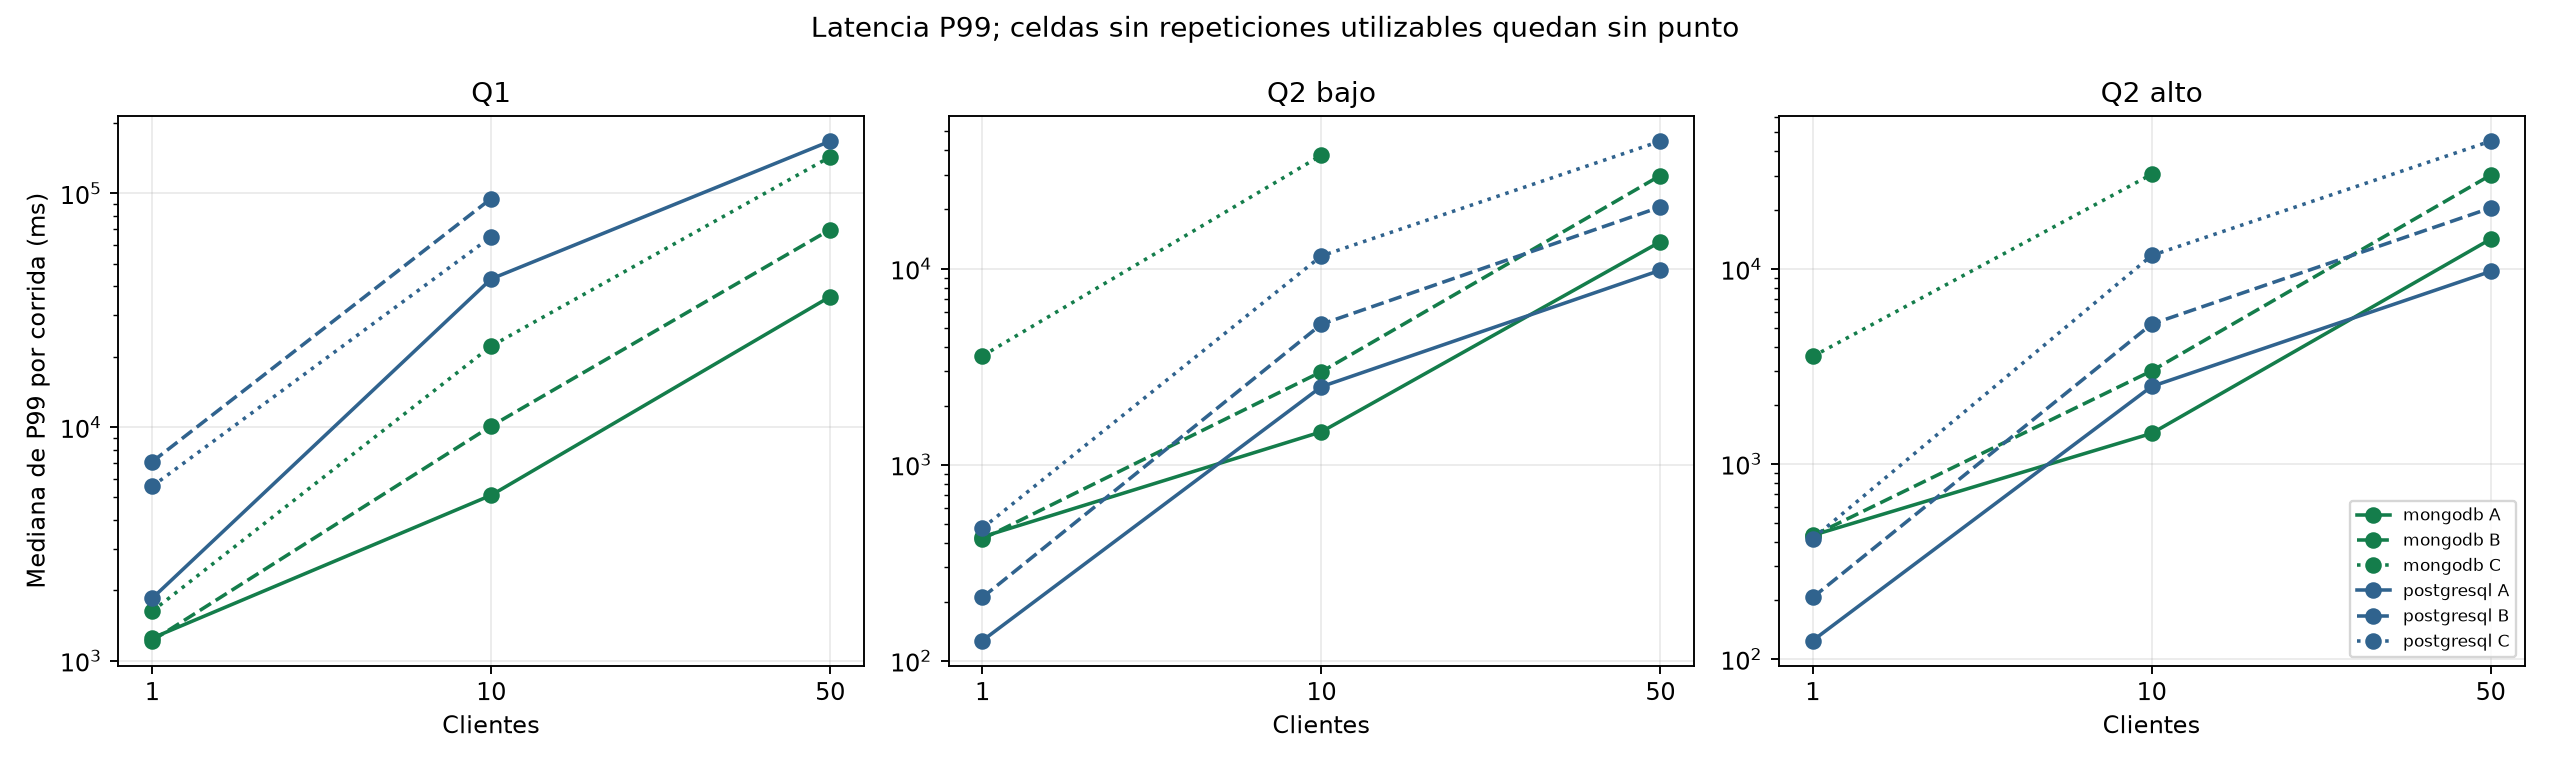
\includegraphics[width=\textwidth,height=0.68\textheight,keepaspectratio]{../resultados/graficas_agricola/p99_concurrencia.png}\par\small\refstepcounter{figure}\addcontentsline{lof}{figure}{\protect\numberline{\thefigure}Tiempo de respuesta y número de clientes}\textbf{Figura \thefigure. Tiempo de respuesta y número de clientes}\end{center}
Mediana de P99 por escenario. La escala vertical es logarítmica y los escenarios sin repeticiones utilizables no tienen punto. Q2 bajo representa sin disco en MongoDB y 4 MB en PostgreSQL; Q2 alto representa con disco y 64 MB, respectivamente. Permite observar cómo cambia el tiempo de respuesta de las consultas más lentas al aumentar el número de clientes. En una escala logarítmica, distancias iguales representan multiplicaciones, no incrementos iguales.
\end{minipage}\par

\begin{minipage}{\textwidth}
\begin{center}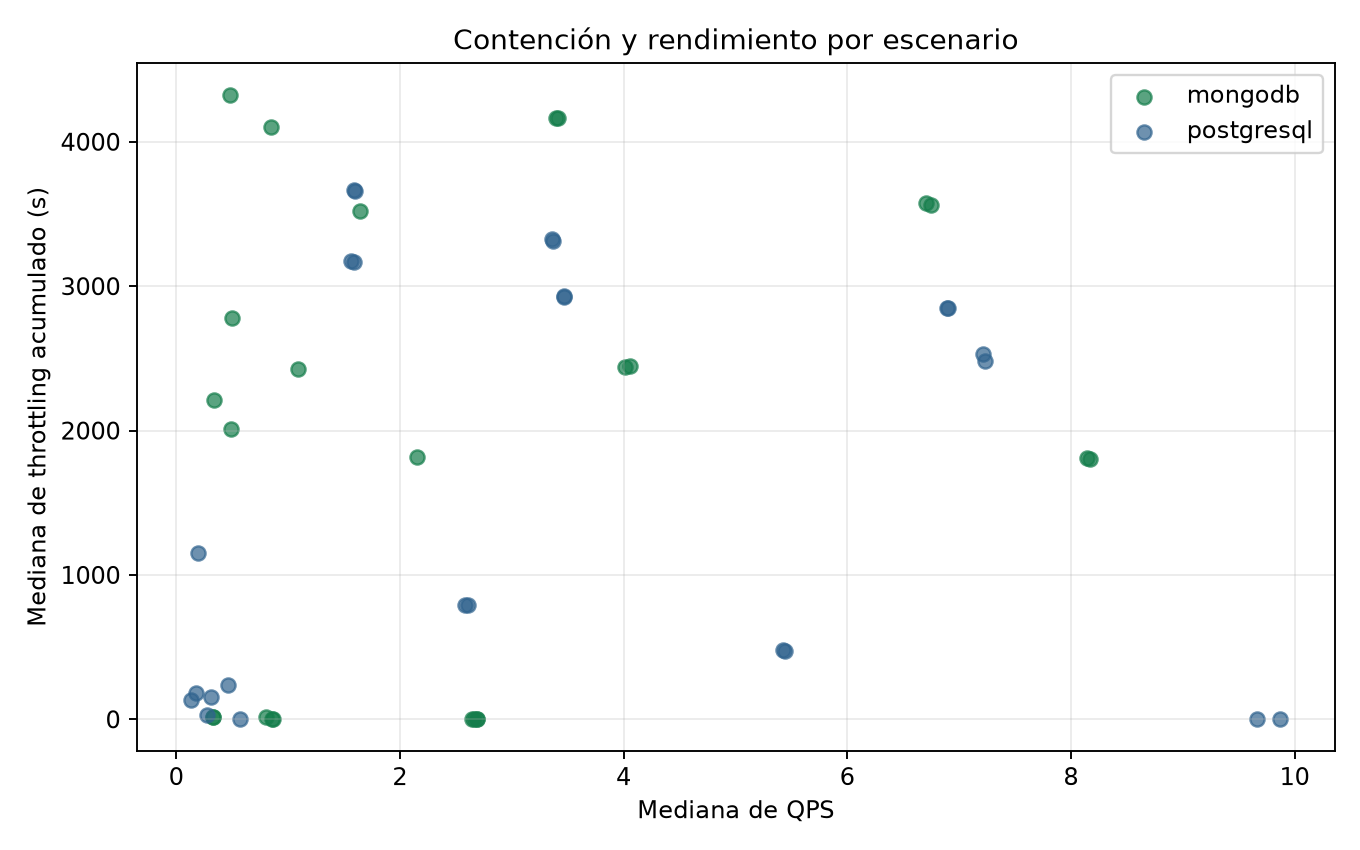
\includegraphics[width=\textwidth,height=0.68\textheight,keepaspectratio]{../resultados/graficas_agricola/throttling_qps.png}\par\small\refstepcounter{figure}\addcontentsline{lof}{figure}{\protect\numberline{\thefigure}Rendimiento y limitación del procesador}\textbf{Figura \thefigure. Rendimiento y limitación del procesador}\end{center}
Relaciona las consultas completadas por segundo con el tiempo acumulado en que se limitó el uso del procesador (throttling). Ayuda a observar si ambos valores aparecen juntos en los escenarios medidos; por sí sola no demuestra que uno cause el otro.
\end{minipage}\par

\begin{minipage}{\textwidth}
\begin{center}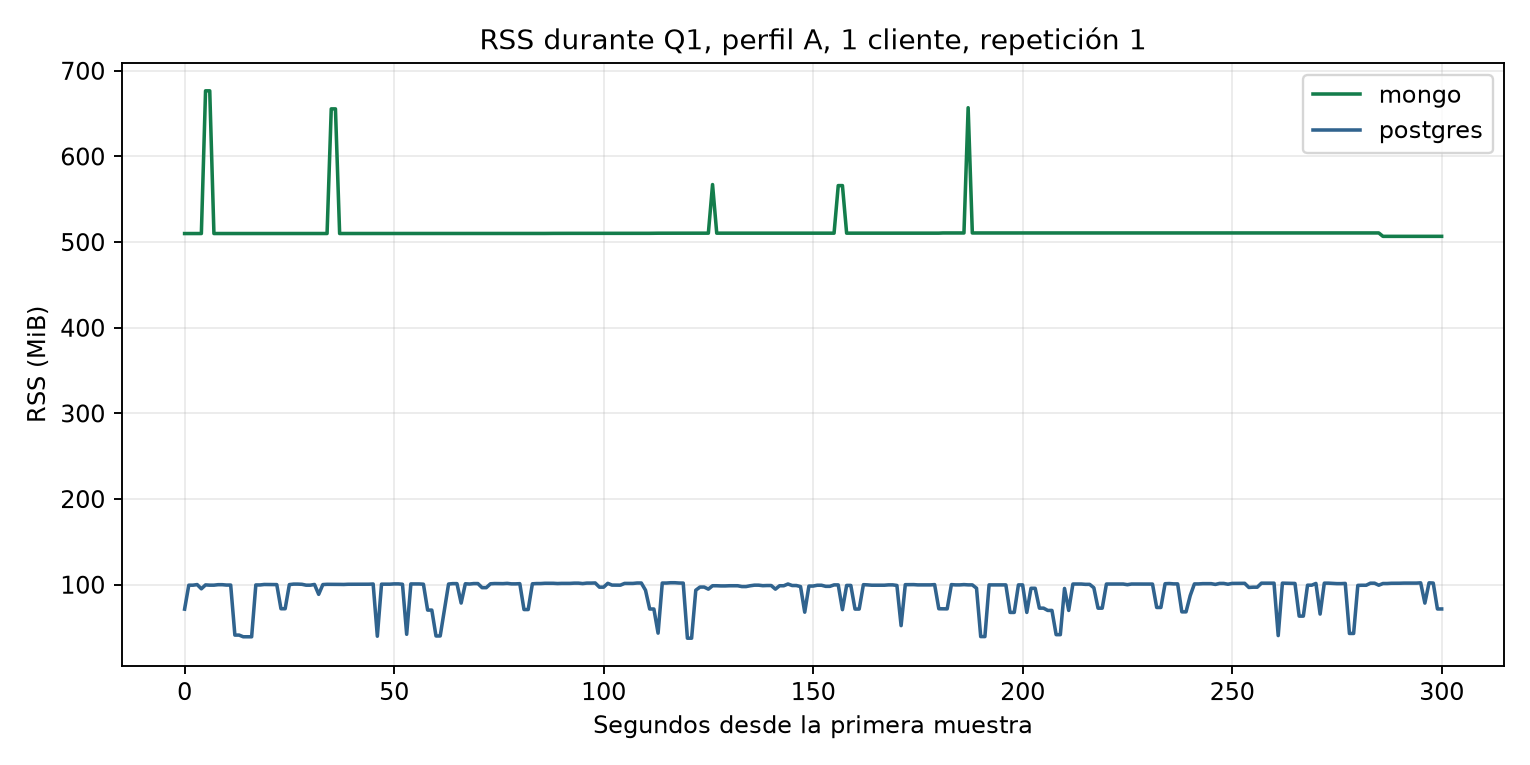
\includegraphics[width=\textwidth,height=0.68\textheight,keepaspectratio]{../resultados/graficas_agricola/rss_ejemplo.png}\par\small\refstepcounter{figure}\addcontentsline{lof}{figure}{\protect\numberline{\thefigure}Memoria residente durante una corrida}\textbf{Figura \thefigure. Memoria residente durante una corrida}\end{center}
Muestra cómo cambia con el tiempo una medida de la memoria residente (RSS) en Q1, perfil A y un cliente, durante la primera repetición de cada motor. Las ejecuciones fueron separadas y se alinearon por tiempo relativo. El RSS mostrado no equivale al uso total de memoria.
\end{minipage}\par

\section*{5. Planes de ejecución}
\addcontentsline{toc}{section}{5. Planes de ejecución}
Los planes de \texttt{resultados/\allowbreak{}planes\_\allowbreak{}agricola/\allowbreak{}} se obtuvieron después de la matriz, con perfil A, como validación puntual; no son mediciones de rendimiento de la matriz. En MongoDB, Q1 mostró \texttt{COLLSCAN} sobre 500.000 documentos y no reportó uso de disco en ese plan. Q2 mostró \texttt{IXSCAN} sobre fecha y examinó 249.767 documentos, con \texttt{usedDisk=false} en las dos variantes observadas.

En PostgreSQL, el plan Q1 con 4 MB mostró lectura secuencial, expansión de lotes y ordenamiento \texttt{external merge}, con bloques temporales. Los planes Q2 de 4 y 64 MB mostraron \texttt{Seq Scan} y \texttt{top-N heapsort}, sin bloques temporales en esas ejecuciones. Un plan puntual no demuestra que todas las repeticiones o cargas concurrentes se comporten igual.


\subsection*{Qué muestran los planes y qué no muestran}
Un plan de ejecución es una descripción de los pasos elegidos por el motor para obtener el resultado. Puede mostrar si recorrió una colección completa, utilizó un índice, ordenó datos o generó archivos temporales. Su utilidad es complementar las mediciones: explica el camino observado en una ejecución, pero no confirma por sí solo la causa de cada diferencia de rendimiento.

En la comprobación posterior, MongoDB recorrió la colección completa para Q1; esto es coherente con una consulta que debe examinar lotes de numerosos documentos antes de agruparlos. Para Q2 utilizó un índice de fecha y después aplicó el resto de la operación. El uso de índice no implica que todos los documentos leídos formen parte del resultado final.

PostgreSQL mostró en Q1 un recorrido secuencial y un ordenamiento externo con bloques temporales en el plan observado. En Q2 apareció una estrategia para mantener los primeros resultados durante el ordenamiento (top-N heapsort), sin bloques temporales en esas ejecuciones. Los planes se capturaron después de la matriz y con perfil A; no se deben presentar como si fueran el plan de cada repetición o como prueba universal del comportamiento bajo todos los límites.

\section*{6. Interpretación y limitaciones}
\addcontentsline{toc}{section}{6. Interpretación y limitaciones}
\textbf{M1.} En los ejemplos de Q1, el P99 aumenta al crecer la concurrencia. En MongoDB A pasó de una mediana de 1.252 ms con un cliente a 36.106 ms con 50; en PostgreSQL A pasó de 1.853 ms a 166.958 ms. Primero se calculó el P99 de cada repetición y después se tomó el valor central de esos resultados (mediana de percentiles por corrida); no es el P99 de todas las consultas juntas. Estas cifras deben leerse con sus cantidades de muestras, errores y operaciones que quedaron fuera de ventana.

\textbf{M2.} Bajo estas condiciones, PostgreSQL registró spill en las repeticiones utilizables de Q1; el plan puntual también mostró ordenamiento externo. El profiler de MongoDB no detectó spill en las corridas para las que pudo comprobarse, pero una corrida tiene spill desconocido. El OOM observado demuestra un fallo por memoria en una corrida concreta; no establece un umbral universal de producción.

\textbf{M3.} Como referencia parcial, en Q1 con perfil A y un cliente, la mediana de CPU consumida durante la ventana de 300 segundos fue 305,1 segundos de CPU en MongoDB y 406,4 en PostgreSQL; la mediana del RSS máximo fue 653,3 MiB y 102,4 MiB, respectivamente. Los segundos de CPU pueden superar el tiempo de pared cuando se usan varios núcleos. Estas cifras representan consumo del contenedor en la ventana, no por documento.

No se registró de manera fiable el número de documentos examinados en cada consulta de la matriz. Por ello no calculamos una cifra precisa de CPU o memoria por cada 1.000 documentos procesados. Los planes puntuales son evidencia útil, pero no justifican asignar su conteo a todas las repeticiones y concurrencias.

Otras limitaciones incluyen datos sintéticos simplificados, cambios de criterios de telemetría y de tamaño del profiler durante la ejecución, posible interferencia del equipo anfitrión y diferencias de instrumentación entre motores. La limpieza de caché de Linux no garantiza vaciar los buffers internos ni la caché de Windows. La medición de spill en PostgreSQL usa logs de archivos temporales en una ventana ampliada, por lo que algunos archivos cercanos a los límites pueden pertenecer al calentamiento o al cierre de consultas.

\section*{7. Recomendaciones}
\addcontentsline{toc}{section}{7. Recomendaciones}
Para una carga semejante a la estudiada, conviene probar ambos motores con las consultas y datos propios antes de seleccionar uno. Es importante medir también los errores y las operaciones que no terminan en la ventana, y no dimensionar recursos solo con QPS o P99 de corridas exitosas.

Para ordenar o agrupar datos, revisar planes e índices y controlar memoria por operación y concurrencia. En contenedores con poca memoria, limitar el número de clientes simultáneos puede reducir la presión, pero el valor adecuado debe medirse para cada sistema. Para futuros experimentos, registrar documentos examinados por operación, capturar resultados que cruzan el fin de ventana y fijar desde el principio los criterios de calidad y la capacidad del profiler.


\subsection*{Cómo utilizar los resultados}
Para elegir una configuración conviene observar conjuntamente velocidad, tiempos de respuesta y estabilidad. Un escenario con QPS alto puede ser poco adecuado si algunas consultas tardan demasiado o si la aplicación no puede tolerar errores. Del mismo modo, un escenario que completa sus consultas usando disco puede ser útil, pero requiere considerar el costo de ese acceso y el espacio disponible.

Antes de trasladar las cifras a otro sistema sería necesario repetir la prueba con datos, consultas, índices y concurrencia representativos. También convendría mantener estable la instrumentación, registrar las consultas que atraviesan el cierre de la ventana y medir los documentos examinados por operación. Esto permitiría responder M3 con una base más sólida y reducir la incertidumbre de los percentiles de muestras pequeñas.

La evidencia disponible distingue la información del caso agrícola de las ejecuciones anteriores utilizadas para preparar el proyecto. Los archivos de la matriz y sus resúmenes son la referencia para los valores incluidos aquí; los registros locales de diagnóstico ayudan a investigar incidencias, pero no sustituyen el CSV consolidado.

\clearpage\normalfont\sloppy\section*{Evidencia y reproducibilidad}
El código, los resultados consolidados y la evidencia versionada se encuentran en el \href{https://github.com/uzzigg/Bases-de-datos-orientadas-a-documentos}{repositorio del proyecto en GitHub}. Los archivos locales señalados abajo no forman parte del repositorio.
\addcontentsline{toc}{section}{Evidencia y reproducibilidad}
\begin{itemize}
\item Datos sintéticos y generación: \texttt{agricola/\allowbreak{}generar\_\allowbreak{}dataset.py}; manifiesto local \texttt{Otros/\allowbreak{}dataset\_\allowbreak{}agricola/\allowbreak{}manifiesto.json}. Huella SHA-256 del archivo agrícola: \texttt{2f73f8a70f7d59b4\allowbreak{}ef0e6f932a725000\allowbreak{}c7b7be2e0368ec77\allowbreak{}4c6358e03d2b9d1a}.
\item Consultas y validación: \texttt{agricola/\allowbreak{}} y \texttt{resultados/\allowbreak{}validacion\_\allowbreak{}agricola\_\allowbreak{}detallada.json}.
\item CSV de las 162 corridas: \texttt{resultados/\allowbreak{}matriz\_\allowbreak{}agricola.csv}; SHA-256 \texttt{68842a8d9b398386\allowbreak{}549cf26a6b89b6e8\allowbreak{}4352fc1e995858ee\allowbreak{}45b28f853ed25d33}.
\item Análisis reproducible: \texttt{scripts/\allowbreak{}analizar\_\allowbreak{}resultados.py}; resultados \texttt{resultados/\allowbreak{}analisis\_\allowbreak{}agricola.json} y \texttt{resultados/\allowbreak{}resumen\_\allowbreak{}agricola.csv}.
\item Planes agrícolas y gráficas: \texttt{resultados/\allowbreak{}planes\_\allowbreak{}agricola/\allowbreak{}} y \texttt{resultados/\allowbreak{}graficas\_\allowbreak{}agricola/\allowbreak{}}.
\item Evidencia cruda, intentos descartados y bitácora: \texttt{Otros/\allowbreak{}} y \texttt{contexto/\allowbreak{}}, guardados localmente y excluidos de Git.
\end{itemize}

\clearpage
\section*{Anexo: guía breve para consultar los resultados}
\addcontentsline{toc}{section}{Anexo: guía breve para consultar los resultados}
Esta guía reúne las unidades y claves que aparecen en las tablas. Su propósito es ayudar a localizar un resultado y comprender qué información aporta cada columna.

\textbf{Motor y consulta.} MongoDB y PostgreSQL son los sistemas comparados. Q1 agrupa lotes por país y cultivo; Q2 obtiene las cosechas con mayor peso. Las etiquetas de Q2 distinguen las opciones de disco en MongoDB y los límites de memoria de trabajo en PostgreSQL.

\textbf{Perfil y clientes.} A, B y C identifican los límites aplicados al contenedor. Los valores 1, 10 y 50 indican cuántos clientes realizan consultas de forma simultánea. Cada combinación se intentó tres veces.

\textbf{N.} Indica cuántas de las tres repeticiones aportaron datos a la mediana. Un valor 2/3 significa que se resumieron dos resultados; 0/3 indica que no hay una mediana utilizable. Los detalles de los intentos permanecen en el CSV.

\textbf{QPS.} Es el número de consultas completadas por segundo. Se usa para describir rendimiento, pero debe leerse junto con los tiempos de respuesta y los estados. No describe por sí solo cuánto tarda cada consulta.

\textbf{P95 y P99.} Son tiempos expresados en milisegundos. Un P95 de 1.000 ms indica que el 95 \% de los tiempos incluidos en ese cálculo quedó en 1.000 ms o menos. Los valores de las tablas son medianas de los percentiles calculados por repetición y excluyen las operaciones que cruzaron el final de la ventana.

\textbf{CPU s.} Son segundos acumulados de restricción del procesador (throttling), no el tiempo total empleado en ejecutar la consulta ni el porcentaje de uso. La suma puede superar la duración de la ventana, por lo que no debe leerse directamente como segundos de reloj transcurridos.

\textbf{Estados.} Una repetición puede terminar normalmente (ok), utilizar disco temporal (spill), registrar un error (error) o agotar memoria (oom). Una casilla desconocida de spill significa que faltó evidencia para determinarlo; no debe tratarse como ausencia de uso de disco.

\textbf{Archivos.} La matriz consolidada conserva los registros originales y el resumen contiene las medianas, mínimos y máximos. Los planes describen ejecuciones puntuales posteriores. Para comprobar un valor o una incidencia se debe empezar por la celda y sus tres repeticiones, y después consultar los registros y planes correspondientes.


\clearpage
\section*{Anexo: análisis detallado de repeticiones}
\addcontentsline{toc}{section}{Anexo: análisis detallado de repeticiones}
Las tablas generales resumen cada escenario con una mediana. Esa presentación facilita la comparación, pero puede ocultar cuántos tiempos de respuesta hubo detrás de cada resultado. A continuación se muestran dos ejemplos extraídos del análisis agrícola para explicar cómo revisar las repeticiones individuales. En ambos casos se trata de Q1 con perfil A y 50 clientes.

\subsection*{Cantidad de tiempos disponibles para calcular percentiles}
La columna «tiempos completos» cuenta las consultas que comenzaron y terminaron dentro de la ventana de medición. La columna «cruzaron el cierre» reúne las operaciones que atravesaron el final de esa ventana y quedaron fuera del cálculo de percentiles. El número de operaciones completadas usado para el rendimiento puede incluirlas; por ello no es necesariamente igual al número de tiempos que alimentan P95 y P99.

\par\begin{minipage}{\textwidth}\refstepcounter{table}\addcontentsline{lot}{table}{\protect\numberline{\thetable}Tiempos disponibles en Q1, perfil A, 50 clientes}\begin{center}\textbf{Tabla \thetable. Tiempos disponibles en Q1, perfil A, 50 clientes}\par\small
\begin{tabular}{lrrrr}\toprule
Motor y repetición & Completadas & Tiempos completos & Cruzaron & Estado \\ \midrule
MongoDB 1 & 499 & 449 & 50 & ok \\
MongoDB 2 & 492 & 442 & 50 & ok \\
MongoDB 3 & 489 & 439 & 50 & ok \\
PostgreSQL 1 & 54 & 4 & 50 & spill \\
PostgreSQL 2 & 66 & 16 & 50 & spill \\
PostgreSQL 3 & 54 & 4 & 50 & spill \\
\bottomrule\end{tabular}\end{center}\end{minipage}\par

La diferencia de tamaños de muestra es importante. En las tres repeticiones de MongoDB hubo más de 400 tiempos completos en cada una; en PostgreSQL hubo 4, 16 y 4. Por tanto, el P99 de PostgreSQL para este escenario es especialmente sensible a los pocos tiempos incluidos. Esta tabla no permite reconstruir los valores de P99 ni decidir cómo se comportaron las consultas excluidas, pero muestra por qué deben interpretarse con cautela.

En el resultado consolidado se reportaron medianas de P99 de 36.105,7 ms para MongoDB y 166.957,9 ms para PostgreSQL. Esas cifras describen los percentiles calculados con los tiempos incluidos, no el comportamiento conocido de todas las operaciones. También se observó uso de disco temporal en las tres repeticiones de PostgreSQL de esta celda. Con estos datos no es posible asignar por separado cuánto de la diferencia se debió al disco, a la CPU o a otros factores.

Este ejemplo ilustra por qué un resultado completo necesita más de una cifra: el tiempo, la cantidad de muestras, la concurrencia, el perfil y el estado de la repetición aportan información distinta. El archivo de análisis conserva además los identificadores de cada corrida, lo que permite regresar a la evidencia correspondiente.

\subsection*{Una repetición con evidencia incompleta}
En MongoDB, Q2 sin disco, perfil A y 10 clientes, la primera repetición terminó con estado de error por falta de registros del mecanismo de diagnóstico (profiler). La segunda y la tercera quedaron en estado ok. La siguiente tabla muestra un dato distinto al de tiempos de respuesta: el número de registros esperados del profiler que no se encontraron.

\par\begin{minipage}{\textwidth}\refstepcounter{table}\addcontentsline{lot}{table}{\protect\numberline{\thetable}Evidencia de profiler para MongoDB Q2 sin disco}\begin{center}\textbf{Tabla \thetable. Evidencia de profiler para MongoDB Q2 sin disco}\par\small
\begin{tabular}{lrrl}\toprule Repetición & Tiempos completos & Registros faltantes & Estado \\ \midrule
1 & 2.527 & 2.326 & error \\
2 & 2.438 & 0 & ok \\
3 & 2.428 & 0 & ok \\
\bottomrule\end{tabular}\end{center}\end{minipage}\par

La primera repetición sí contiene tiempos de consulta, pero su evidencia de uso de disco quedó incompleta. Por esa razón no se incluyó en la mediana de rendimiento del escenario y su indicador de spill se conserva como desconocido. Las otras dos repeticiones sí forman la mediana publicada, por lo que la columna N muestra 2/3. No se trata de una conclusión de que el motor utilizó o dejó de utilizar disco en la repetición afectada.

\subsection*{Lectura de una falla por memoria}
En PostgreSQL, Q1, perfil B y 50 clientes, el estado de las tres repeticiones fue error, oom y error. En la segunda se observó que el contador de procesos terminados por falta de memoria aumentó de 1 a 2 durante la corrida. Ese cambio es la evidencia para señalar un evento de falta de memoria en esa repetición concreta.

Las tres repeticiones se conservan en la matriz, pero ninguna tiene un estado incluido en las medianas de rendimiento del informe. Por eso en la tabla de PostgreSQL con perfil B la celda aparece con N = 0/3 y guiones. La ausencia de una mediana impide compararla numéricamente con otra que sí terminó; al mismo tiempo, la falla es un resultado de estabilidad relevante para explicar los límites de esa configuración.

\section*{Anexo: ruta de consulta y verificación}
\addcontentsline{toc}{section}{Anexo: ruta de consulta y verificación}
La evidencia del proyecto se puede consultar por niveles. No es necesario interpretar todos los archivos al mismo tiempo: el lector puede empezar con una pregunta concreta y seguir la ruta que corresponda.

\textbf{1. Identificar el escenario.} En las tablas del reporte se localizan el motor, el perfil, la consulta o variante y la cantidad de clientes. Estos cuatro elementos identifican la combinación que se quiere estudiar. Para Q2 hay que mantener visible la opción del motor, porque permitir disco y asignar memoria de trabajo son controles diferentes.

\textbf{2. Revisar las repeticiones.} El CSV consolidado contiene una fila por repetición, con el estado y las métricas registradas. El resumen agrupa esas filas y muestra cuántas repeticiones se usaron, además de valores centrales, mínimos y máximos. Una comparación justa debe considerar tanto la mediana como el número de repeticiones que la respaldan.

\textbf{3. Consultar los detalles.} El análisis agrícola contiene información por corrida sobre muestras de latencia, operaciones que cruzaron el cierre, errores y datos de diagnóstico. Permite entender, por ejemplo, por qué una celda muestra 2/3 o por qué una mediana de P99 basada en pocas consultas necesita cautela.

\textbf{4. Contrastar el resultado de las consultas.} El archivo de validación detallada reúne las comprobaciones de Q1 y Q2: sumas y conteos, diferencia máxima de promedios, pesos del Top-1000 y situación de los empates. Su función es respaldar la comparación funcional; no mide el tiempo de respuesta de la matriz.

\textbf{5. Revisar un plan.} Los planes guardados muestran qué operaciones eligieron los motores en las ejecuciones de comprobación posteriores. Son útiles para localizar recorridos completos, índices, ordenamientos y uso de archivos temporales observado en esas pruebas. Para no confundir evidencia, se debe recordar que fueron capturados con perfil A después de la matriz.

\textbf{6. Consultar la bitácora local.} Las carpetas locales de trabajo contienen detalles adicionales de preparación e incidencias. No forman parte de los archivos versionados del repositorio. Si otra persona necesita repetir el experimento, debe contar con el código y los datos necesarios, además de conocer las condiciones y limitaciones anotadas en el informe.

\subsection*{Límites de la reproducción}
Reproducir el procedimiento significa volver a preparar datos y consultas equivalentes, aplicar los perfiles y registrar cada repetición. No significa que los valores numéricos deban ser idénticos en cualquier equipo. Las versiones de los motores, los recursos del anfitrión, el estado de las cachés y la instrumentación pueden modificar las cifras.

Para una nueva ejecución sería conveniente fijar desde el inicio las condiciones de monitoreo, guardar las operaciones que terminan después del cierre y registrar el número de documentos examinados por operación. Así se podrían investigar las diferencias de percentiles y calcular con mayor fundamento el consumo solicitado por M3. Las decisiones tomadas durante esta ejecución se presentan en el método, de modo que un lector pueda distinguir el protocolo previsto de lo que ocurrió realmente.

\section*{Referencias}
\addcontentsline{toc}{section}{Referencias}
\begin{itemize}
\item Manuales de la actividad: \texttt{playbook.pdf} y \texttt{playbook\_\allowbreak{}sesion.pdf}, proporcionados para el experimento.
\item MongoDB, \href{https://www.mongodb.com/docs/manual/tutorial/manage-the-database-profiler/}{Database Profiler}: funcionamiento y sobrecarga del profiler.
\item PostgreSQL, \href{https://www.postgresql.org/docs/current/using-explain.html}{Using EXPLAIN}: interpretación de planes y buffers.
\item Prometheus, \href{https://prometheus.io/docs/prometheus/latest/querying/basics/}{Querying basics}: consultas y vectores de rango.
\end{itemize}
\end{document}
